\chapter{Dictionary Learning on Graph Data with Weisfieler-Lehman sub-tree kernel and KSVD.}\label{ch:graph_sparse}

\section{Introduction}\label{intro}
Graph data is usually highly dimensional and defined in a non-euclidean form. Hence, typical processing methods defined on euclidean spaces cannot be used on graph data. Graph embedding methods convert the graph data into a vector representation while trying to preserve original graph properties\cite{Cai2018}.%\cite{Chen2020, Cai2018}.
Graph embedding methods can be classified as node embedding, edge embedding, hybrid embedding, and whole graph embedding. In literature, a distinction is made between graph representation learning and graph embedding\cite{Cai2018, Chami2022}, where graph representation does not require the final vector to be low-dimensional. In this paper, we focus on whole graph embedding, where each entire graph is represented as a vector\cite{Maddalena2021}. The vector representation can be used to compare graph similarity for important tasks, including classification and clustering. The main challenges in whole graph embedding are how to capture the properties of a whole graph and how to make a trade-off between expressiveness and efficiency\cite{Cai2018}. Several methods have been proposed for whole graph embedding, including matrix factorization, deep learning, edge reconstruction, graph kernel, and generative models\cite{Cai2018, Maddalena2021}.

Graph2Vec is a popular neural network-based architecture for graph embedding\cite{Narayanan2017}. Some advantages of Graph2Vec are that the model is trained in an unsupervised manner, the learned model is task agnostic, the algorithm is data-driven, and resulting vectors capture structural equivalences. Graph2Vec utilizes the non-linear Weisfeiler-Lehman (WL) kernel\cite{weisfeiler1968reduction},
which is shown to outperform other linear kernels\cite{shervashidze2011weisfeiler, Yanardag2015}. WL kernel is used to rename the nodes using a hash value that represents a rooted sub-graph on the given node. These sets of node names are viewed as a set of words in a document. The techniques from the Natural language processing (NLP) domain are borrowed for learning an embedding. Doc2Vec is based on Word2Vec\cite{Mikolov2013}, in which a feed-forward neural network (NN) ``SkipGram'' model with negative sampling is used to learn a representation of word sequences\cite{Le2014}. Using the SkipGram model, the nodes with similar neighborhoods are embedded closer together\cite{Rong2014}. The Graph2Vec is implemented in the ``KarateClub'' python package\cite{Karateclub}\footnote{\url{https://karateclub.readthedocs.io/en/latest/}}. An overview of the implementation of the Grap2Vec is shown in Fig.\ref{fig: G2V}, where a vocabulary of sub-tree structures is generated using a WL sub-tree kernel and a Doc2Vec model is trained on the selected vocabulary. 

Some disadvantages of Graph2Vec are the nonlinearity of the learned embedding and the generated sub-tree structures. Due to the nonlinearity, it is difficult to identify which sub-tree structures are contributing to the similarities and differences among graphs. Hence, we propose a linear representation model to replace the Doc2Vec NN architecture. Further, the SkipGram model is capable of embedding only a single node, rather than node combinations. In addition, the SkipGram model considers the neighborhood of the nodes, which depends on an arbitrary node numbering scheme that may not generalize between graphs in a given application.

\begin{figure}[!t]
\centerline{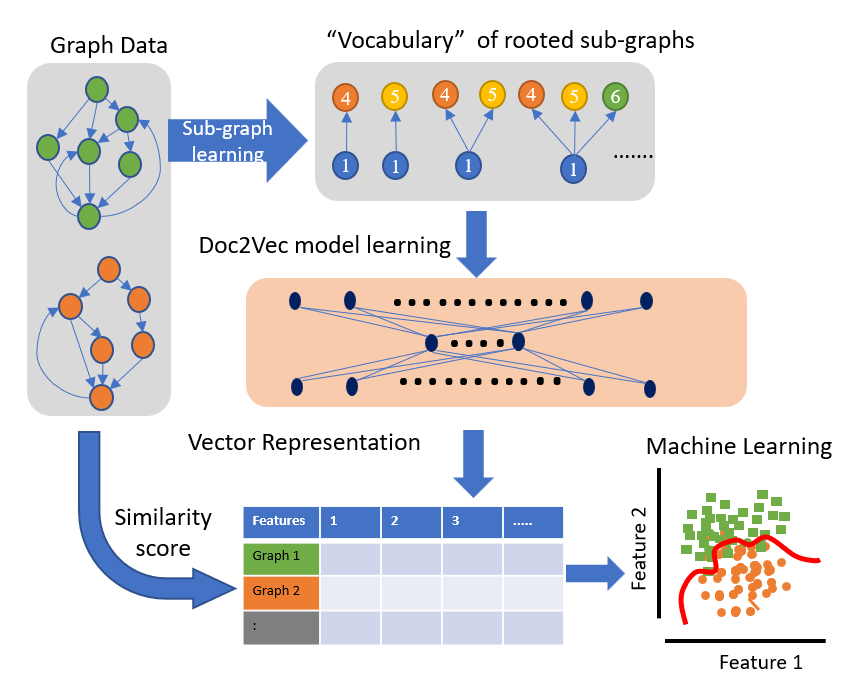
\includegraphics[width=0.9\columnwidth]{figures/Gaph2Vec.png}}
\caption{Graph2Vec pipeline overview}\label{fig: G2V}
\end{figure}

\begin{figure}[!t]
\centerline{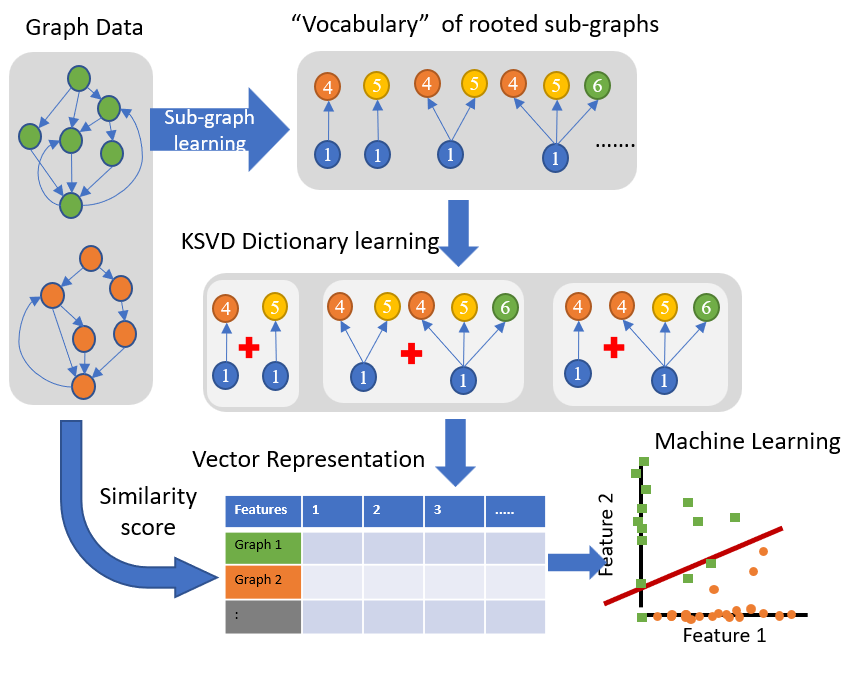
\includegraphics[width=0.9\columnwidth]{figures/GraphKSVD.png}}
\caption{Proposed WL+KSVD pipeline overview}\label{fig: GKSVD}
\end{figure}

Sparse representation is a technique used to learn a dictionary that lies in the original feature domain and calculate a sparse representation using a linear combination of a few dictionary elements (atoms)\cite{Elad2010}. %\cite{Elad2010, Zhang2015}.
The main advantages of using sparse representation are linearity and sparsity: the learned embedding consists of linear combinations of sub-tree structures; sparse representations allow using low-order classifcation models due to the low VC dimension\cite{Neylon2006}. Sparse representation was originally introduced in the signal and image processing domains, however recently it has been utilized in graph-related processes. Several methods have been proposed to represent graph signals on a fixed graph topology with sparse representations with theoretical guarantees\cite{Yankelevsky2019}. %\cite{Subbareddy2019, Thanou2013, Zhang2021, Yankelevsky2020}.
Recent work by Matsuo et al.\cite{Matsuo2019} develops a method to represent different network topologies with sparse representation. However, their work is still limited by requiring graphs to be undirected and requiring all topologies to have the same number of nodes.

To address the shortcomings in sparse vector-based graph representations, we introduce a framework to incorporate WL sub-tree kernel with sparse representation methods specifically aimed at machine learning classification tasks. Our framework allows sparse representation to be applied to graphs with different topologies and different numbers of nodes. In addition, the input graphs can be directed and can incorporate node features. An overview of the proposed WL+KSVD pipeline is shown in Fig.\ref{fig: GKSVD}. The proposed method has the flexibility to swap different dictionary learning and graph kernel methods in the framework. The method is tested against several similar graph embedding methods with benchmark datasets. Finally, the python implementation of the framework and the experiments are currently available on Github\footnote{\url{https://github.com/BMW-lab-MSU/WL-KSVD.git}}.

\begin{figure}[!t]
\centerline{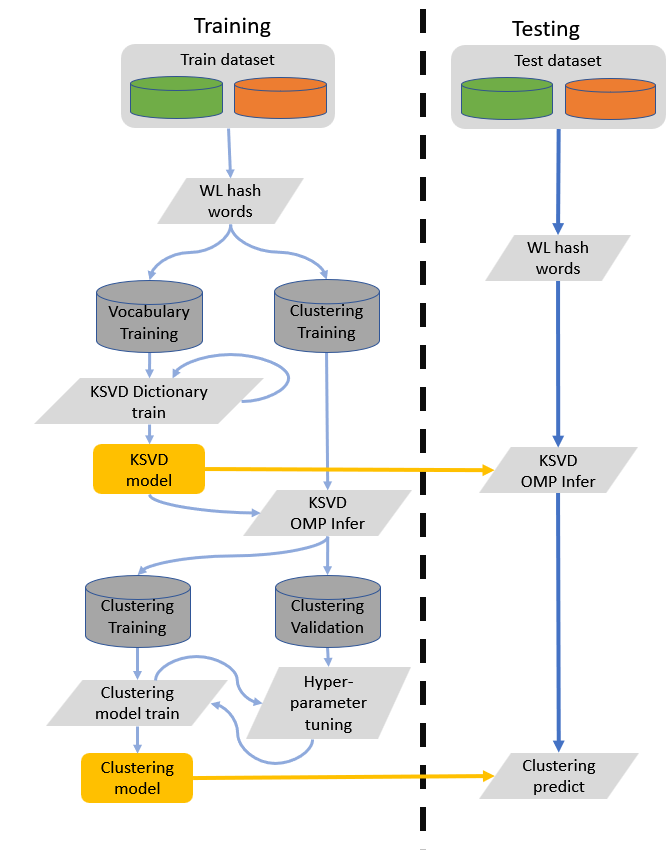
\includegraphics[width=0.9\columnwidth]{figures/Workflow.png}}
\caption{Evaluation Workflow}\label{fig: workflow}
\end{figure}
